\section{考察}
\subsection{初期バージョンとバージョン2の比較}
初期バージョンとバージョン2では,後者の方がプログラム自体の行数は多い.しかしそれは動的メソッドを実装するにあたって重複分をまとめた関数を増やしたためである.今後新たに数学関数を実装していくと仮定した場合,既に重複分がまとめてある関数を実装するならば,プログラムに書き足すのは実装する数学関数についての関数のみであるので,かなり簡潔で済む.
一方で,既に実装されているものと重複がないまたは出力が同じでない場合,初期バージョンと同じようにプログラムを書くことになる.加えて初期バージョンはMapleに送る式を必ず書くため,Mapleでのプログラムに慣れた人には初期バージョンの方で実装する方が容易かもしれない.

\begin{figure}[htbp]\begin{center}
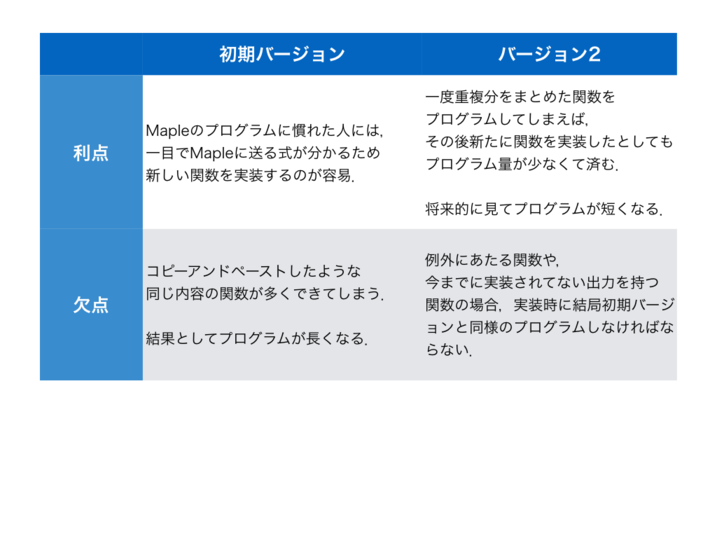
\includegraphics[width=10cm,bb= 0 0 737 553]{../figs/./mapleruby_eringi.009.png}
\caption{各バージョンの利点,欠点}
\label{default}\end{center}\end{figure}
\subsection{maplerubyを使うメリット,デメリット}
最大のメリットは,Rubyだけで桁数の大きい計算や複雑な数学関数を必要とする計算を完結させられることである.今後扱える関数を増やせば,利用者がMapleについて詳しくない人でもRubyのプログラムを書くだけで数値計算処理が可能になるだろう.またRubyライブラリにあるTest::Unitと並行して使用すれば,求めたい解が分かっている際に自分が書いたプログラムで正しく解が導けるのかテストすることも可能である.

デメリットは大きく3つある.1つ目はRubyは無償で使えるがMapleは有償である点.よって,利用者が限られてしまう.2つ目はRMapleクラスの中に使いたい関数が実装されてない場合,自力で関数を実装するかMaplerubyクラスを直に使うかしなければならない点.よってプログラミングにMapleの知識が必要になってくるためメリットで挙げた「Rubyプログラムを書くだけで数値計算処理が可能になる」のが難しくなる.3つ目は桁数の大きい計算は確かにできるものの,処理に多少時間がかかってしまう点.処理速度を上げようと思うとMaple自体の処理速度を上げなければならない.

